% !TeX root = ./Dyplom.tex

\chapter{Analiza wymagań projektowych}
\label{sec:analiza}

\section{Wymagania funkcjonalne}
	Wymagania funkcjonalne określają wymagania dotyczące pożądanego zachowania systemu.
	Definiują, jakie usługi ma oferować i jak ma reagować na określone dane wejściowe.
	Wyszczególniono następujące wymagania funkcjonalne:
	\begin{enumerate}
		\item System zawiera katalog albumów
		\item Albumy da się wyświetlać wraz ze szczegółami
		\item Każdy album można oceniać oraz dodawać recenzję
		\item Istnieje możliwość dodawania nowych albumów
		\item Wyszukiwanie albumów korzysta z bazy zewnętrznego serwisu
		\item Możliwość rejestracji i logowania
		\item Wybór pomiędzy ciemnym i jasnym motywem aplikacji
	\end{enumerate}

\section{Wymagania niefunkcjonalne}
	Wymagania te określają właściwości systemu, jego ograniczenia i standardy w jakich pracuje.
	Wymagania systemu spełniającego założenia projektowe są następujące:
	\begin{enumerate}
		\item Aplikacja powinna być obsługiwana przez obecne wersje przeglądarek
		\item Do poprawnego działania wymagane jest połączenie z Internetem
		\item Aplikacja powinna być napisana w sposób umożliwiający łatwe dodawanie nowej funkcjonalności
		\item Dane użytkowników są przechowywane w bezpieczny sposób
	\end{enumerate}

\section{Przypadki użycia}
	Na rysunku~\ref{fig:useCase} przedstawiono diagram przypadków użycia użytkownika aplikacji.
	Zawarte zostały główne funkcjonalności skupiające się na przeglądaniu albumów i dodawaniu recenzji.
	W ten sposób wyszczególniono następujące przypadki użycia:
	\begin{enumerate}
		\item Dodanie oceny albumu\\
			Przypadek użycia dotyczy akcji dodania oceny do albumu.
			Dodawanie opisowej recenzji jest opcjonalne, dlatego ujęte zostało jako opcjonalny, rozszerzający przypadek użycia.

		\item Wyszukanie albumu z bazy Last.fm\\
			Aby dodać ocenę do albumu należy wyszukać odpowiedni album wpisując jego nazwę lub wybrać z najpopularniejszych albumów podanego artysty.
			Wyszukiwarka korzysta z API Last.fm, jednak nie wymaga konta na tym serwisie.

		\item Logowanie\\
			Dodawanie ocen dostępne jest tylko dla zalogowanych użytkowników.
			Przeglądanie albumów i recenzji nie wymaga konta.
		
		\item Rejestracja\\
			Jeśli użytkownik nie ma jeszcze utworzonego konta, a chce dodawać oceny to może się zarejestrować.

		\item Przeglądanie listy albumów\\
			Użytkownik może przeglądać wszystkie albumy, do których zostały dodane oceny.
			Po kliknięciu w album przenoszony zostaje do widoku wyświetlającego wszystkie dane albumu.

		\item Zarządzanie ustawieniami\\
			Przypadek użycia opisujący zmianę ustawień aplikacji, które są unikalne dla każdego użytkownika.
			Na chwilę obecną możliwa jest zmiana motywu głównego aplikacji (jasny/ciemny).

	\end{enumerate}
	
	\begin{figure}[ht]
		\centering
			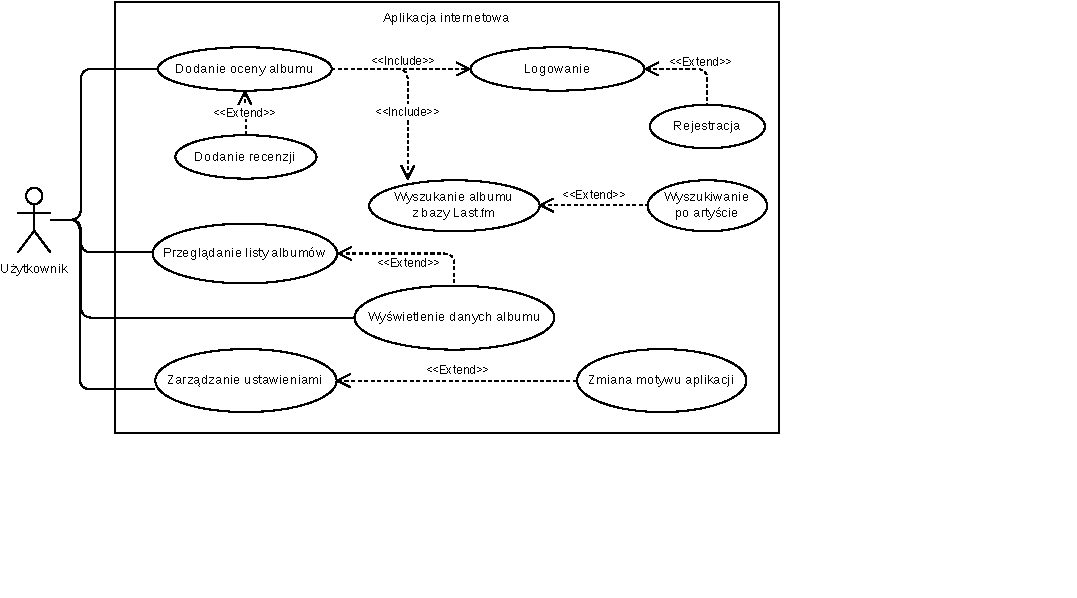
\includegraphics[width=\linewidth]{rys02/useCase.pdf}
		 \caption{Diagram przypadków użycia}
		 \label{fig:useCase}
	\end{figure}

\section{Założenia projektowe}
	Całość aplikacji zaprojektowana zostanie ze wsparciem platformy Docker.
	Każda odrębna część systemu zamknięta będzie we własnym wirtualnym kontenerze:
	\begin{enumerate}
		\item strona internetowa typu Single-Page Application:\\
			Architektura SPA pozwala tworzyć strony, które w swoim działaniu bardziej przypominają tradycyjne aplikacje komputerowe.
			Podczas interakcji użytkownika ze stroną fragmenty widoku są dynamicznie odświeżane zamiast przeładowywania całej strony.
			Dodatkowo strona powinna przechowywać w pamięci zapytania do serwera aby minimalizować czas oczekiwania na dane.

		\item serwer uwierzytelniający użytkowników:\\
			Strona internetowa działa po stronie klienta, przez co możliwa jest znaczna ingerencja w dane.
			Aby minimalizować zagrożenia, zaimplementowane zostanie uwierzytelnianie użytkowników wykorzystujące bezpieczny protokół.
			Wykorzystany standard powinien zapewnić zarówno uwierzytelnianie jak i autoryzację.

		\item serwer dostępowy do danych aplikacji:\\
			Grafowy dostęp do bazy danych zaimplementowany zostanie za pomocą GraphQL\@.
			Serwer umożliwiać będzie pobieranie danych stosując zapytania w języku GraphQL\@.
			Dzięki temu relacje między danymi przedstawione są w postaci grafu,
			co pozwala formować skompilowane zapytania bez potrzeby tworzenia dedykowanych kontrolerów i modeli DTO po stronie API\@.

		\item baza danych:\\
			Baza danych powinna umożliwiać przechowywanie relacji między obiektami w taki sposób,
			aby możliwe było reprezentowanie danych w postaci grafu.

		\item serwer dostarczający odwrócone proxy:\\
			Z racji tego, że użytkownicy będą przekierowywani między główną stroną, a stroną do uwierzytelniania,
			adresy serwerów zarejestrowane będą w odwróconym proxy.
			Będzie to również główny punkt dostępu do aplikacji, który będzie kierował ruchem.
			Dodatkowo, będzie obsługiwał szyfrowanie przesyłanych danych protokołem HTTPS\@.

	\end{enumerate}
